\documentclass{acm_proc_article-sp}
\usepackage[english,ngerman]{babel}
\usepackage[utf8]{inputenc}
\usepackage{abbrevs}
\usepackage{url}

\usepackage[
pdftex,colorlinks=false,
bookmarks=true,b
ookmarksopen=true,
bookmarksopenlevel=0,
plainpages=false,
bookmarksnumbered=true,
hyperindex=false,
pdfstartview=,
pdfauthor={Jan Philip Bernius, Ekaterina Sebina},
pdftitle={Monitoring: Ambari and Chukwa}
]{hyperref}


%% ABBREVIATIONS
\newabbrev\isds{Internet-scale Distributed Systems (ISDS)}[ISDS]
\newabbrev\amb{Apache \textit{Ambari}}[\textit{Ambari}]
\newabbrev\chuk{Apache \textit{Chukwa}}[\textit{Chukwa}]


\begin{document}
\title{Monitoring: Ambari and Chukwa}
\subtitle{Seminar: Internet-scale Distributed Systems}

\numberofauthors{2}

\author{
% 1st. author
\alignauthor
Jan Philip Bernius\\
       \affaddr{Technische Universität München}\\
       \affaddr{Department of Computer Science}\\
       \email{\href{mailto:janphilip.bernius@tum.de}{janphilip.bernius@tum.de}}
% 2nd. author
\alignauthor
 Ekaterina Sebina\\
       \affaddr{Technische Universität München}\\
       \affaddr{Department of Computer Science}\\
       \email{\href{mailto:katie.sebina@tum.de}{katie.sebina@tum.de}}
}

\date{15 July 2015}

\maketitle

%TODO REMOVE!
\nocite{*}

\begin{abstract}
%TODO: Abstract

The main topic of this paper is the concept of monitoring in distributed systems presented in \ambshort and \chukshort. 
Our thesis is to explain the core difference between \ambshort and \chukshort, based on the monitoring process and find the most suited environment for each application. 
The emphasis is on the benefits that each application is offering to the current technology processes and systems. 
With a short introduction on the architectures of both applications, the core field of use can be explained. 
\ambshort's main function is to simplify the use of Hadoop, while \chukshort's is to optimise the analysis and storage on Hadoop clusters. 	
\end{abstract}

\category{H.3.4}{Systems and Software}{Distributed systems}
\category{C.2.3}{Network Operations}{Network monitoring}


\terms{Documentation, Experimentation, Measurement, Performance, Reliability, Security, Standardization}

\keywords{Hadoop, Monitoring, Map and Reduce, Ambari, Chukwa, Apache, OpenSource, Java, Internet-Scale, Distributed Systems, Cluster, Cloud}

\noindent\rule{84mm}{0.4pt}

\section{Introduction}
%TODO: Introduction
As internet applications are increasing, more and more servers are getting integrated into distributed systems.\cite{Dinu2011} Applications need to be run on multiple servers parallel to fulfil their responsibilities. Further the number of running nodes will vary based on user number and activity.\cite{Jammes2012} As these systems get impossible to administer by hand, automating the process is very important.\cite{Jammes2012} Systems tend to fail from time to time, therefore it is very useful to notice failure and fix occurring problems in advance. Jerome Boulon, Principle Engineer at Yahoo! and PPMC in the Chukwa team, stated, that ``Large distributed systems can fail in complicated and subtle ways.''~\cite{Boulonb} Monitoring allows to notice, archive failures. It provides Developers and System Administrators with details about occurring failures and errors. The following paper will describe and compare two monitoring Systems, \amb and \chuk. Both systems use \hadoop and the \mr method as basic component.\cite{ApacheSoftwareFoundation2015}


\subsection{Definitions}

\textit{Monitoring} is a process, which controls, interacts and manages other processes and systems. It has the ability to locate, prevent and repair failures in advance. It is an important strategy for availability and security of procedures. Monitoring is always running parallel to activities and gives the user the ability of a faster failure cooper, that possibly people could do.\cite{Jammes2012}

\amb is an open source framework that allows to control, manage, provide and install Hadoop Cluster easily from the included Web-Interface. It simplifies the use of Hadoop.\cite{Hortonworks2013}

\chuk is a large-scale Log Collection and Management System. It is specialised to collect Log files as well as Application Metrics from distributed Clusters.

\subsection{Structure of this paper}
First, the concepts of Hadoop and Map Reduce~(\ref{subsec:Hadoop}) are explained, these concepts are the basis of the techniques introduced in this paper. 
Second, the concept of monitoring~(\ref{subsec:ConceptMonitoring}) is introduced and two interpretations and implementations, Apache Systems \amb and \chuk are explained~(\ref{subsec:Implementation}) in more detail. 
Third, a comparison~(\ref{subsec:Differentiation}) is made and, lastly, a conclusion~(\ref{sec:Conclusion}) is drawn.

\subsection{Literature Review}
As it is highly recommended to document the research and review process,~\cite{brocke09} this paragraph will summarise the research and review process.

The research started on the self description on the project websites and continued using technical documentation, describing the underlying architecture of both systems.
Further, Library Databases, especially \emph{IEEE Xplore} and \emph{EBSCOhost} were utilised to find more in-depth material, including the research these projects are based on. A lot of details about the use and monitoring process of Ambari were found at Hortenworks.
	
\subsection{Hadoop}
\label{subsec:Hadoop}
Hadoop is an open source software by Apache for storing and analysing data.\cite{Dagli2014} It divides and storages Big Data across multiple smaller clusters, by copying them three times with the map and reduce function. This concept implies a high fault tolerance, if one of the clusters fail.\cite{Dagli2014}

Hadoops Architecture is divided in many parts. To understand \amb and \chuk, the three main parts will be enough.\cite{Dagli2014}
  \begin{enumerate}
  	\item Hadoop Clusters are multiple new storage places for the data. They are divided into one master node and several server nodes, that are fulfilling the tasks of the master node.\cite{Dagli2014}
  	\item \hdfs, are file systems that are responsible for storing data across multiple machines.\cite{Dagli2014}
  	\item Map and Reduce is the main function which maps and reduces data till the core mean on all Hadoop clusters.\cite{Dagli2014}
  \end{enumerate}

\subsubsection*{Map Reduce}
The Map and Reduce process is the main function of Hadoop. After the division of data across multiple clusters, it maps similar datasets together into one cluster. 
Later on it analyses and reduces the data till the main sense. This data is getting combined together into the output. \cite{Dagli2014}

Hadoop Users need to implement the rules for the map and reduce process. All the other parts of the function such as sort and store are already available, when Hadoop is getting installed.\cite{Dagli2014}


\amb and \chuk both presuppose a basic understanding of Hadoop as well as the map and reduce function. Both application are powered by Apache and are monitoring processes for Hadoop.They differ in their area of operation of monitoring.\cite{ApacheSoftwareFoundation2015}

\section{Ambari and Chukwa}
Our intension is to show the adavtanges of each application with in a use case to answer the question for with monitroing operation Ambari or Chukwa should be preferd.
\subsection{What is the concept of monitoring and how is it used in general?}
\label{subsec:ConceptMonitoring}

Monitoring is getting popular nowadays. It is a process which is managing, oberserving and intervaining into other processes. Its main goal is to controll the actions, as well as prevent and fix fauliers. Monitoring can be used in diffrent ways, based on the Use-Case field. The most comman areas are large companies that work on diffrent continets togehter and need to develope one product, medicin, in controlling heart dicisses.
\\
 In distributed Systemens, the core aim of monitoring is to fix and prevent faults quicklie. This improves the qualitie of the system and its capabilitie. Monitroing applications usually integreated into the structer of communication in between the distributed systems. By Virus or dengeroucs information that should be send from one computer to an another, monitoring would intervane and stop or divorse the maschine from the whole system, to save the systems healt. 
\subsection{How is the concept of monitoring implemented in Ambari and Chukwa?}
\label{subsec:Implementation}
After defining monitoring and its Use Cases, two Software Solutions for monitoring in an \hadoop environment are introduced.

\subsubsection{Ambari}
\amb is ``the only 100\% open source framework''~\cite{Sako2013} that allows the User to monitor, manage and install Hadoop.\cite{ApacheSoftwareFoundation2015} It has the ability to start, stop and configure Hadoop processes automatically on clusters, without any intervention of the user.\cite{Hortonworks2013} \amb was founded to simplify the use of Hadoop.\cite{Hortonworks2013}

\amb architecture can be divided in connected parts. First the \amb Web which is the main platform for Users to log in and give up request that should be run through Ambari.~\cite{Sako} It builds the main Interface for any interactions between User and Application.\cite{Sako} Through \amb web all the monitoring processes are visualized. 

Secondly, the \amb Server consists out of several components.\cite{Sako} The (REST-) API is connected to different Web applications, the most important one is \amb Web.\cite{Sako} Other interfaces, like Microsoft System Centre, are applications that allow the user to analyse the data. Furthermore the capability of Hadoop or integrate data and conclusions to other programs of the User.\cite{Hortonworks2013} The results of the analysis is accessible through \amb Web on the monitoring screens.\cite{Sako}

The connection between \amb and \hadoop is done by the \amb Agents.\cite{Sako} During setip, \amb Server will install the \amb Agent Software on each host. The Agent will sent a regular heartbeat to the server for communication. The server answers with an instruction for the Agent or sends a confirmation about his current life-status.\cite{Sako} All hosts are connected to the clusters by \hadoop.\cite{Sako}

\begin{figure}
  \centering
  % https://docs.google.com/open?id=1A3TbXPEQeknqWxxX811XHG7pcQOuMEFDmo_hl8LlfYk
  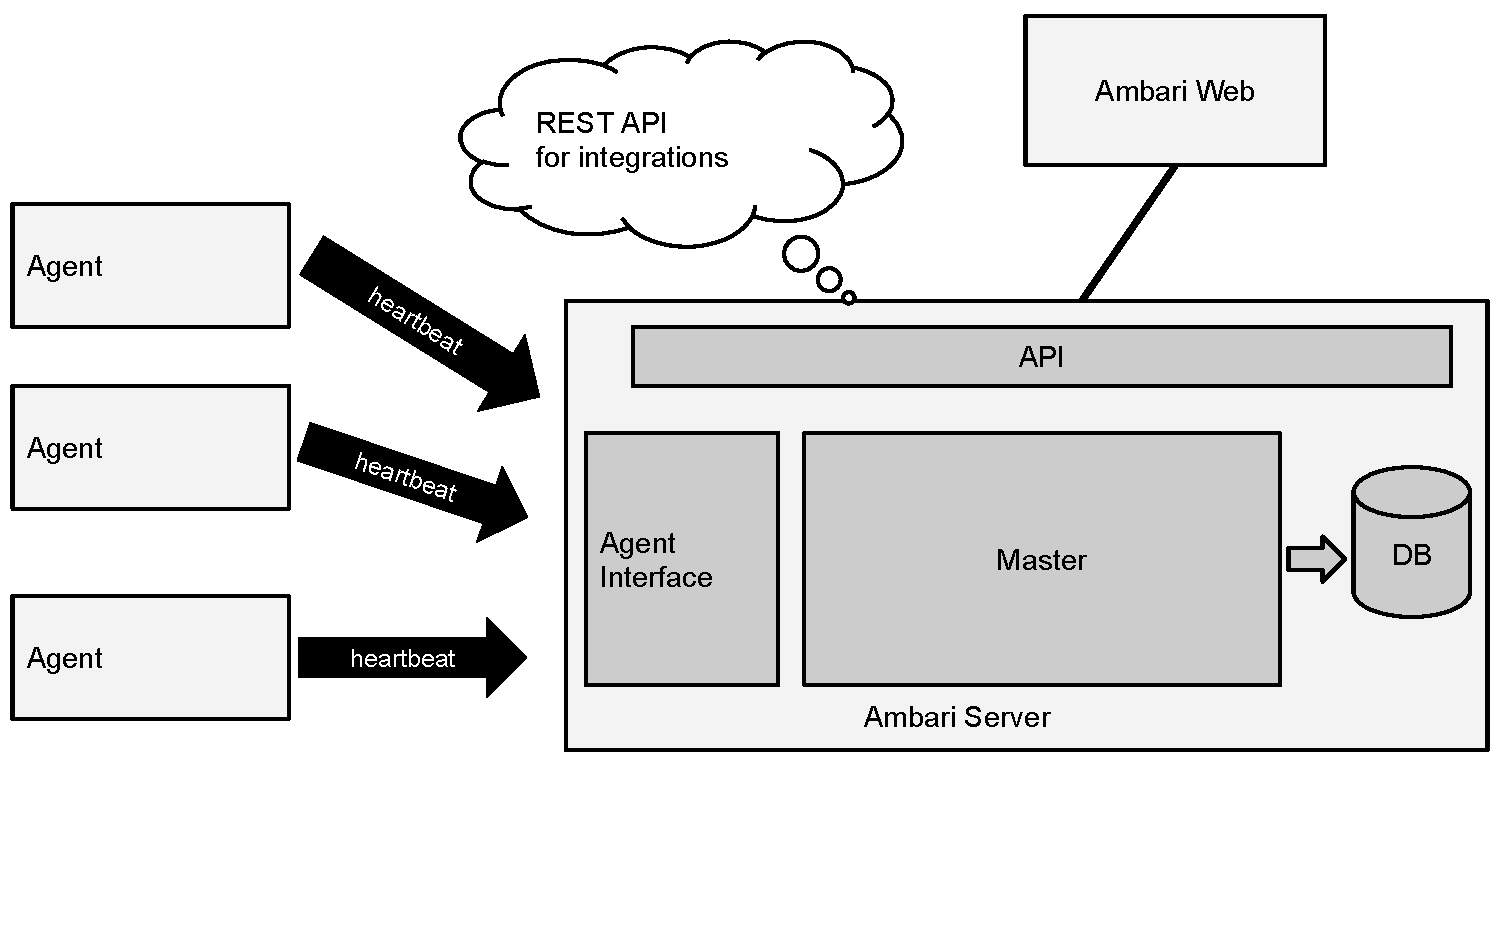
\includegraphics[width=\linewidth,clip=true,trim=0 3cm 0 0]{images/AmbariArchitecture}
  \caption{Ambaris Architecture~\cite{Sako, Sako2013}}
  \label{fig:AmbariArchitecture}
\end{figure}

The concept of monitoring is given in two specific ways with \amb. 
It has knowledge about every nodes health and its data.~\cite{Foley2012} 
It can provide and improve the health situation of a Hadoop cluster and analyse the data in ways there are useful for the user.~\cite{Foley2012} 
The user has an overview on the current situation through the Web application.~\cite{Foley2012} 
\amb divides to monitoring Process in three parts.~\cite{Foley2012} 
The first one is the List of all the Applications \amb is running on each connected cluster. 
It shows the name, status and number of clusters that are ok, and the ones that need to get fixed.~\cite{Foley2012} 
The second part is explaining all the technical details about the application, such as storing space and running time.~\cite{Foley2012} 
The last part is aimed to show illustratively how long and effective an application has been running on a node.~\cite{Foley2012} 
Based on this data the user can give up requests to change the applications or add more clusters into one process, through the API.~\cite{Sako} 
\amb then will install a new application automatically to the cluster. This command is sent as a response to a heartbeat signal from an \amb Agent. \cite{Sako} 
\amb has the ability of installing and giving a breve overlook about the health of the system; its not capable of analysing the data qualitatively.\cite{Sako}


\subsubsection{Chukwa}
\chuklong is ``a data collection system for monitoring and analyzing large distributed systems.''~\cite{Boulona}
It is built to support log handling on scalable Hadoop clusters. 
Further, it allows ``[c]ross system analysis''~\cite{ChukwaPoster} 
\chuk is developed at Yahoo! and ``is built on top of HDFS and Map-Reduce.''~\cite{Rabkin2008a}
Its main non-functional goals are low footprint on System Usage (less than 5\%) and minimal changes to user workflow.~\cite{Rabkin2010}
``All (..) data [is] in one place''~\cite{ChukwaPoster} eventually.

\paragraph{The process}
For processing Log files and Application Metrics, \chuk starts on the producing machine, which is running a \chuk Agent. 
This piece of Java Software is constantly gathering Application Logs and Metrics from pre-configured locations. 
This can be \textit{syslog} as well as an Application specific location. 
Each Source is fetched by a so called \textit{Adaptor}.~\cite{ChukwaAdminAgent}

\begin{figure}
  \centering
  % https://docs.google.com/open?id=11xCUWZ94zbUa4eqhoScjMmfIL2pI-IkDx02qvcCXohY
  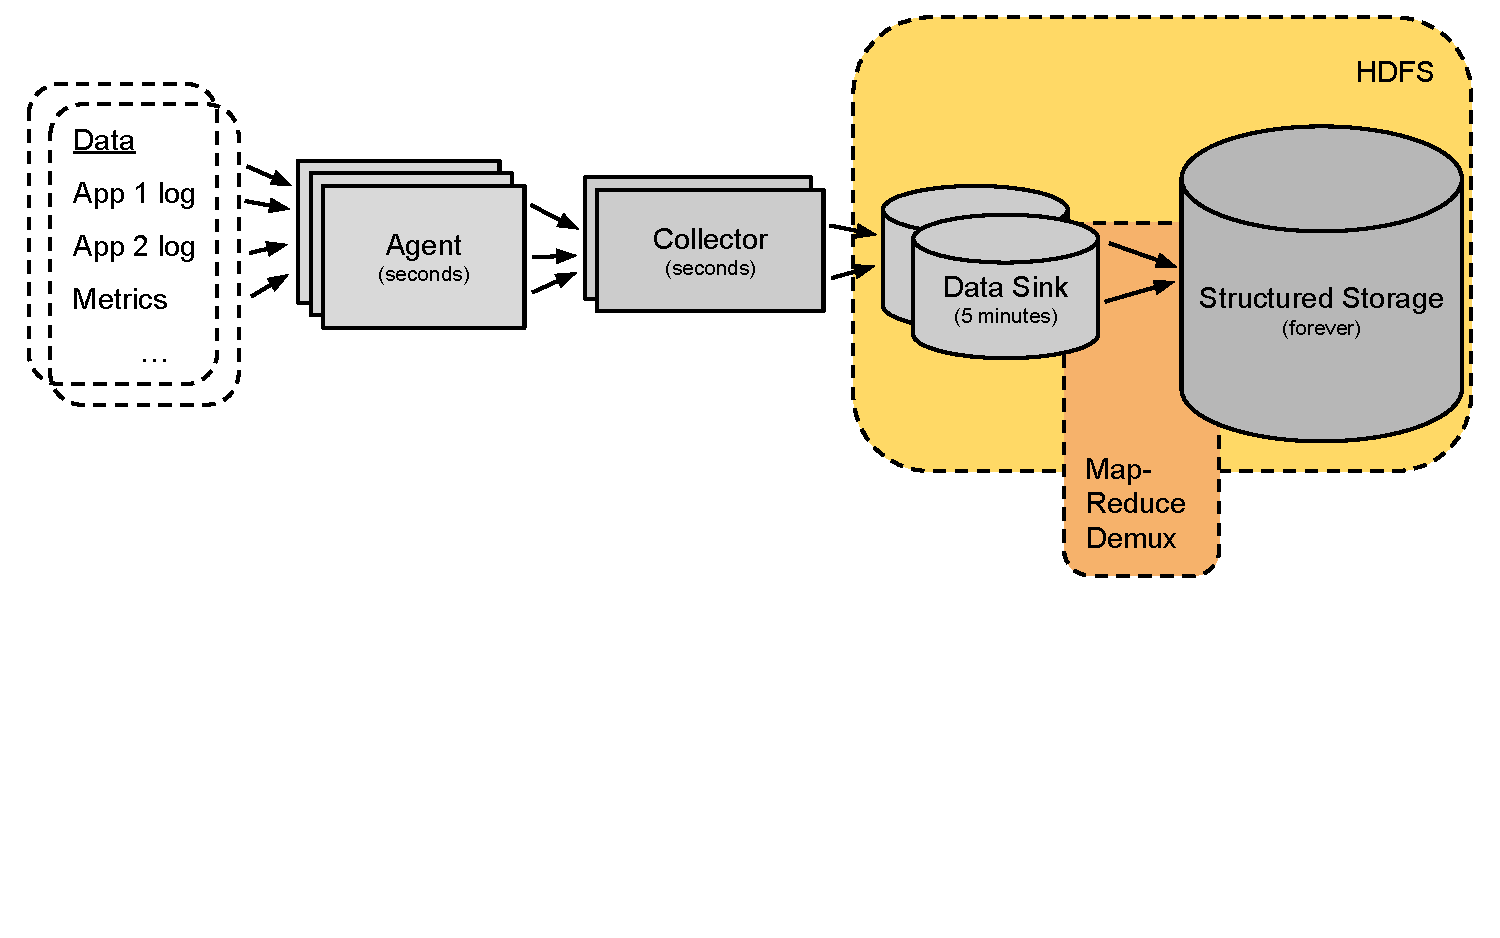
\includegraphics[width=\linewidth,clip=true,trim=0 6cm 0 0]{images/ChukwaArchitecture}
  \caption{Chukwas Architecture~\cite{Rabkin2008}}
  \label{fig:ChukwaArchitecture}
\end{figure}

The Agent is then pushing the data to a so called \textit{Collector}, as described on Figure~\ref{fig:ChukwaArchitecture}.
This is another piece of Java Software, running on a dedicated \chuk instance. 
The \textit{Collector}s job is collecting data from multiple Nodes in the Cluster, as well as archiving and post-processing the data.~\cite{Jose2014}
First, the collected information is stored in \textit{Data Sink} Files. 
Here, data from multiple Nodes gets written in the same file, which can be seen as a Queue for processing.
Every few minutes, the \textit{Data Sink} File is closed. (Files cannot be processed, while data is written to them.)
All available \textit{Data Sink} files will be processed by a pair of Demux \mr jobs.~\cite{Boulona} 


As described by Boulon et al., the \mr processing should produce insights about 
``needs for accounting, capacity planning, performance characterization, utilization'', 
``reduc[e] the number and extent of outages'', 
``reduc[e] the number of false alerts and increasing the value and confidence level of true alerts'' and 
``reduc[e] the time and effort required to identify and resolve cluster issues.''~\cite{Boulonb}

To achieve these goals, ``the first job simply archives all the collected data, without processing or interpreting it. 
The second job parses out structured data from some of the logs, and loads this structured data into a data store.''~\cite{Boulona} 

% reduce can be customised. https://chukwa.apache.org/docs/r0.4.0/programming.html

\paragraph{The Storage}
\label{par:chukStoreage}
The \mr jobs will \demux data out of the \textit{sink} files and into structured storage.~\cite{Boulonb} 
\chuk supports multiple, pluggable storage formats, which ``also aids integration with legacy systems. Chukwa also offers the flexibility to support other data sources, such as syslog or local IPC.''~\cite{Rabkin2010a} 

Currently, \chuk uses \hdfs files, ``one file per cluster, per data type, and time period. (..) [Which is only an] interim solution''~\cite{Boulona} 
The development team is evaluating different data-stores, which are more suitable for the purpose and allow structured querying, also.
Possible storage systems for the future include Hive, HBase or Hypertable. Also local installations of relational Databases might be an option.~\cite{Boulonb} Last option depends on the amount of data stored.

\textit{Hive} is potentially a good fit. It is still based on \hdfs files, but adds a new layer of organisational functionality like ``Organization into Tables'' or a ``SQL like query language over object data stored in Tables.''~\cite{Sarma08}
\subsection{How does Ambari differentiate from Chukwa?}
\label{subsec:Differentiation}

\amb and \chuk are, while both being Monitoring Systems, engineered for different use-cases. 
As stated in \ref{subsec:ConceptMonitoring}, the concept of monitoring allows different applications in the domain of \isds. 

\subsubsection{Ambari}
\amb was founded to simplify the use of Hadoop Systems. It offers management, monitoring and intervening process on Hadoop Clusters.\cite{Hortonworks2013} 

After-all, \amb fulfills two tasks on a \hadoop cluster. 
First, \amb provides metrics about a cluster in general, like number of running hosts, cluster health, overall RAM/CPU Usage, Network Traffic etc. \amb also provides Host specific Metrics.
\\
Second, \amb can perform Actions on the entire Cluster, a group of Hosts or individual hosts. 
%TODO extend on actions

\subsubsection{Chukwa}
\chuk offers extensive data collection capabilities, especially optimised for storing, archiving and analysing ``a large and open-ended set of time series metrics and logs.''~\cite{Boulona}

Different to \amb, \chuk does only perform read operations on the hosts. Its highly configurable Agent will upload all data to the Collector, where processing takes place.


Even though some Use Cases~(\ref{netflix}) show that it is possible, \chuk does not aim to provide Real-Time information. However, after processing is done, the data is available in a structured form and can be stored forever. \mr and \demux also allows automated analysis and error detection as shown in the Use Case~(\ref{netflix}). This allows reporting to responsible System Administrators or Software- Engineers in a efficient manner. It also provides detailed error information, as the related log information is available.

\subsubsection{Comparison}
%TODO rethink if it fits this way
In comparison of both applications, \amb approaches a wilder spectrum out of all \hadoop tasks, while \chuk is specialised on storing and analysing \hadoop Data. Both differ in their core range of use for \hadoop, in connection of monitoring. \amb is not capable of monitoring the actual data value that is stored on the clusters that are getting observed, but it can monitor the health of those.\cite{ApacheSoftwareFoundation2015} While \chuk has the ability to interpret and analyse data on its monitored clusters.

Both Systems offer \emph{complementary} services. \amb can do real-time management of the cluster and provide real-time system status. \chuk will archive system- and Application-Log-Information and put it in structured \hdfs storage.

\section{Conclusion}
\label{sec:Conclusion}
\subsection{Summary}

\subsection{Use Case: Netflix}
One of the most known users of a \chuk derivate is \textbf{Netflix}, who is using \aws to provide their service. A fairly large number of \aws EC2 Instances is deployed, producing about $1.5$ million events per Second during peak hours. This results in about $80$ billion events per day. Most of the events are reflected as log messages, user activity records, system operational data, or any arbitrary data.~\cite{Bae2013}

Netflix is providing lots of its technology as Open-Source software, including their \chuk clone \textit{Suro}. 
Beside integrations with \noss, Suro offers several modifications to \chuk, which ``grew out of what [Netflix] learned from meeting the operational requirements of running in production over the past few years.''~\cite{Bae2013}

Suro goes beyond Chukwas scope of functionality in the following points:
\begin{enumerate}
  \item Suro supports ``arbitrary data formats,''~\cite{Bae2013} which allows more types of application to support advanced logging by Suro. A Plug-in System allows customised serialisation and deserialisation code to be run during processing.
  \item Lots of monitoring metrics are already included within Suro, 
  \item Integrations with other \noss Tools is included within Suro. This makes it especially easy to use Suro in a Cloud Setup, also using other \noss tools.~\cite{GithubNetflixSuro}
  \item \label{itm:SutoMultiDest} Dispatching Events to multiple destinations is available with custom configuration as of flexible architecture.~\cite{Bae2013, GithubNetflixSuro} 
  \item ``Suro supports configurable store-and-forward on both client and collector.''~\cite{Bae2013} Its ``support of flexible retries'' leads to minimised data loss.~\cite{GithubNetflixSuro}
\end{enumerate}
Suro still preserves attributes from \chuk like horizontal scalability as well as ``large number of connections, and high throughput''~\cite{GithubNetflixSuro}

Item~\ref{itm:SutoMultiDest} allows Use-Cases like the one described in Figure~\ref{fig:SuroArchitecture}. 
\label{netflix}
\begin{figure}[hbt]
  \centering
  % https://drive.google.com/open?id=1Nmn-mWvxAwhcB9Vo4nbq0gutnWp0bPcCfBU14KMDVQ8
  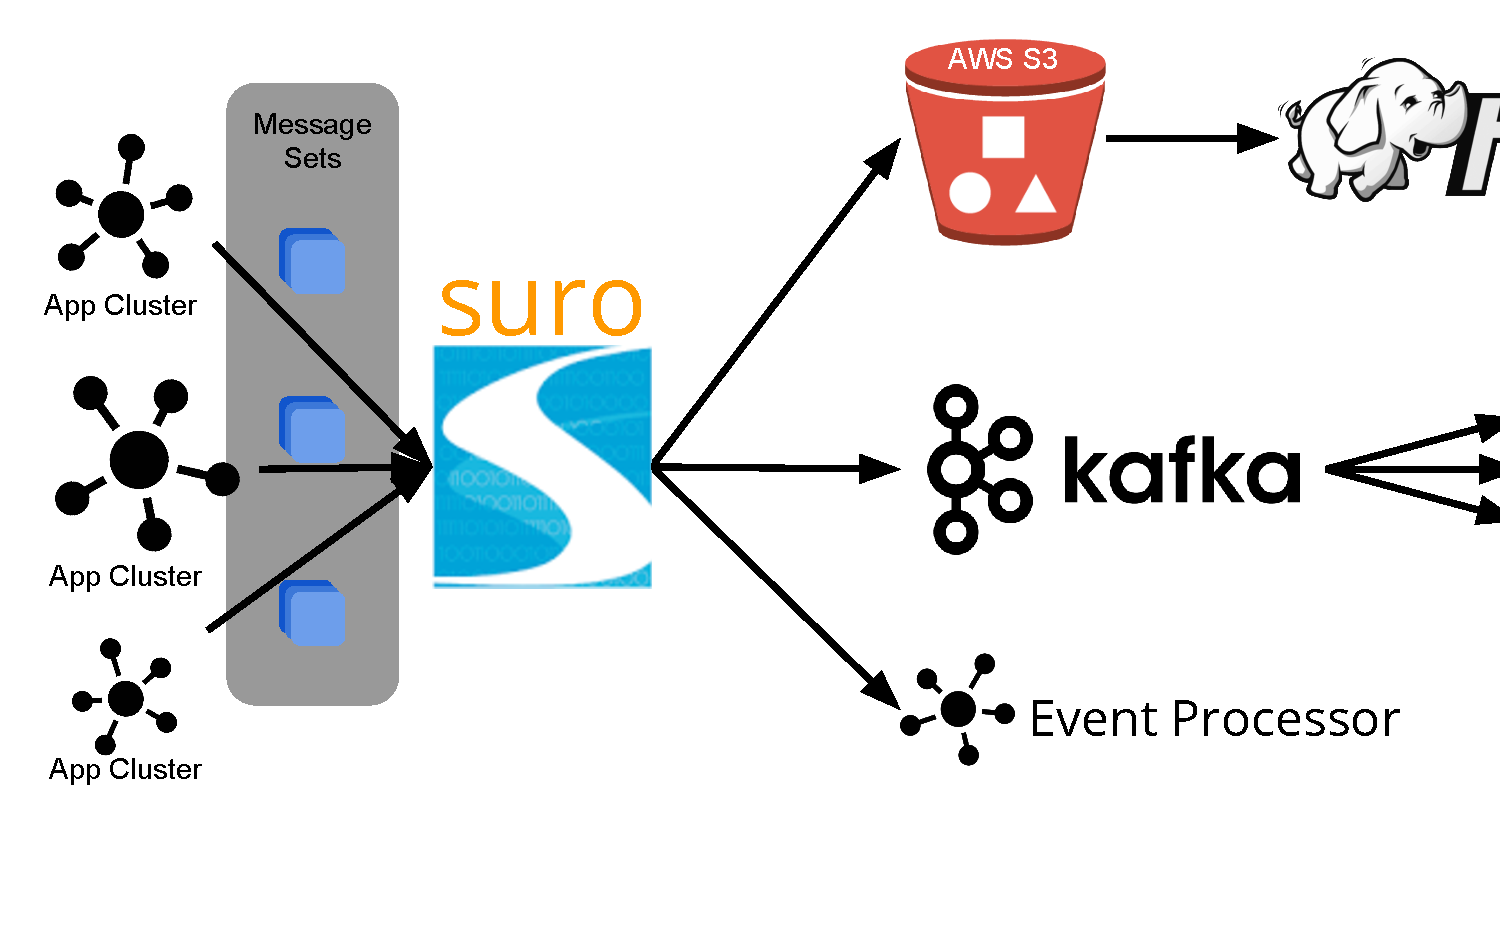
\includegraphics[width=\linewidth,clip=true,trim=5mm 2cm 0 5mm]{images/NetflixSuro}
  \caption{Netflix Suro Architecture~\cite{Bae2013, Harris2013}}
  \label{fig:SuroArchitecture}
\end{figure}

\begin{figure}[hbt]
  \centering
  % https://drive.google.com/open?id=1Nmn-mWvxAwhcB9Vo4nbq0gutnWp0bPcCfBU14KMDVQ8
  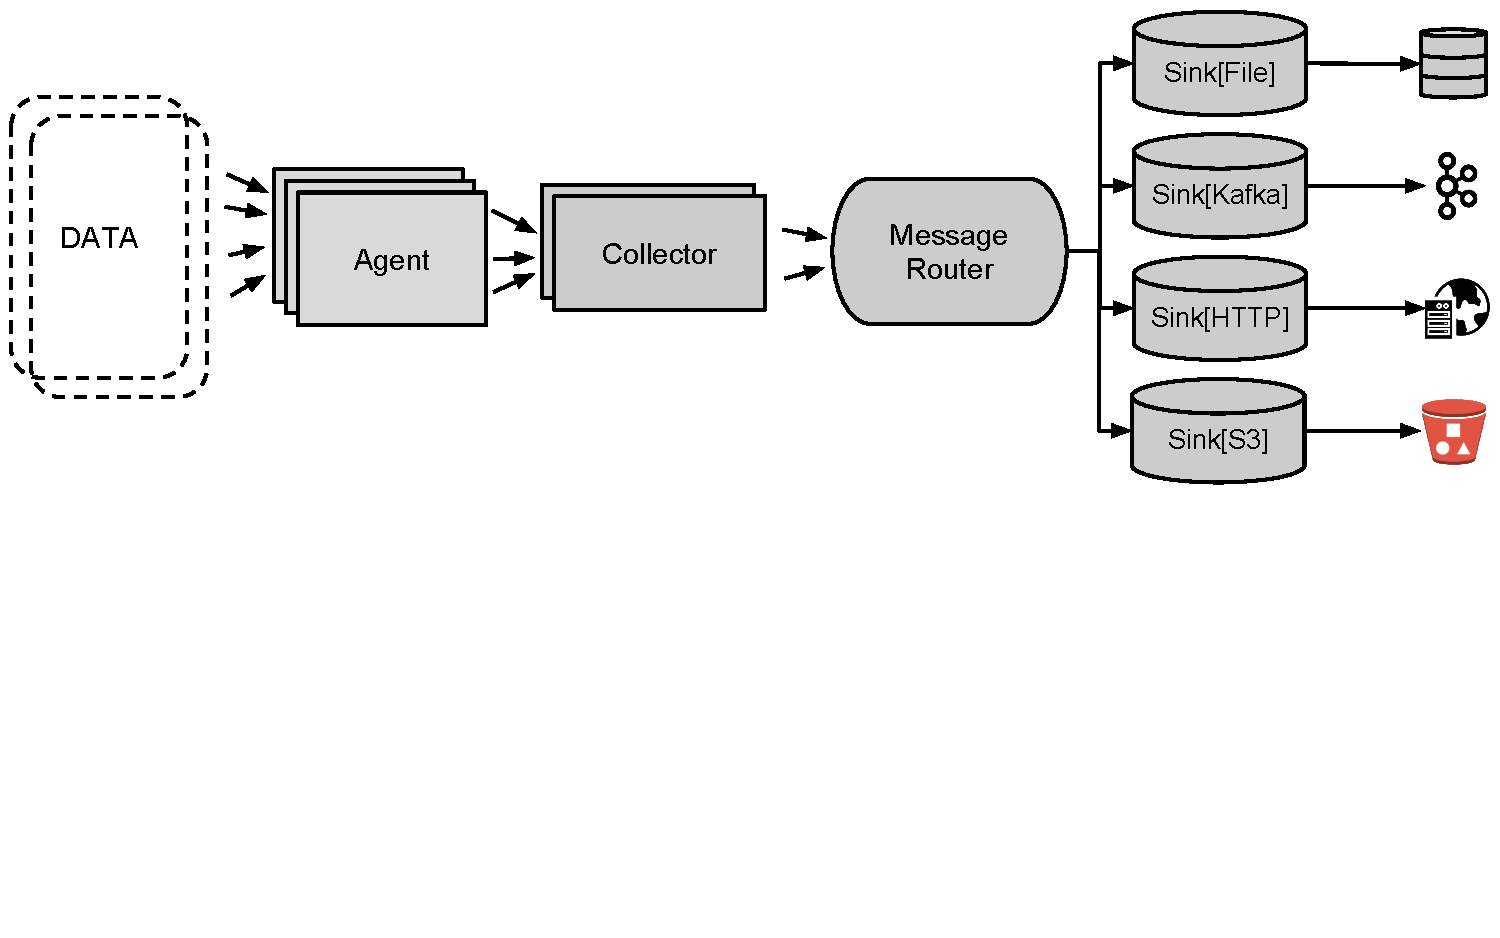
\includegraphics[width=\linewidth,clip=true,trim=0 75mm 0 0]{images/SuroMessageRouter}
  \caption{Netflix Suro Message Router~\cite{Bae2013}}
  \label{fig:SuroMessageRouter}
\end{figure}


\subsection{Future research}
Current research has not shown, in which extend the two systems \amblong and \chuk can be used in an inter-connected manner, complementing each others services. Managing large, internet-scale clusters, consisting of multiple thousand hosts running \hadooplong can be more automated and controlled with Systems like \amb and \chuk in place, not only controlling the current state, but also managing installed components and archiving system-state information.

Further, an improved way of storing Chukwas log data in a more structured way, allowing live querying, is still be to found. Boulon et al. did look into several options so far~\cite{Boulonb}, but this work has to be continued.

Last, but not least, the real-time approach shown in \ref{netflix} may be extended, as the ``recent trend has been in the area of real-time stream processing''~\cite{Bae2013} and will most likely continue in the future.

%TODO: ACKNOWLEDGMENTS are optional
% \section{Acknowledgments}

\bibliographystyle{abbrv}
\bibliography{bibliography}

\end{document}
